\begin{figure}
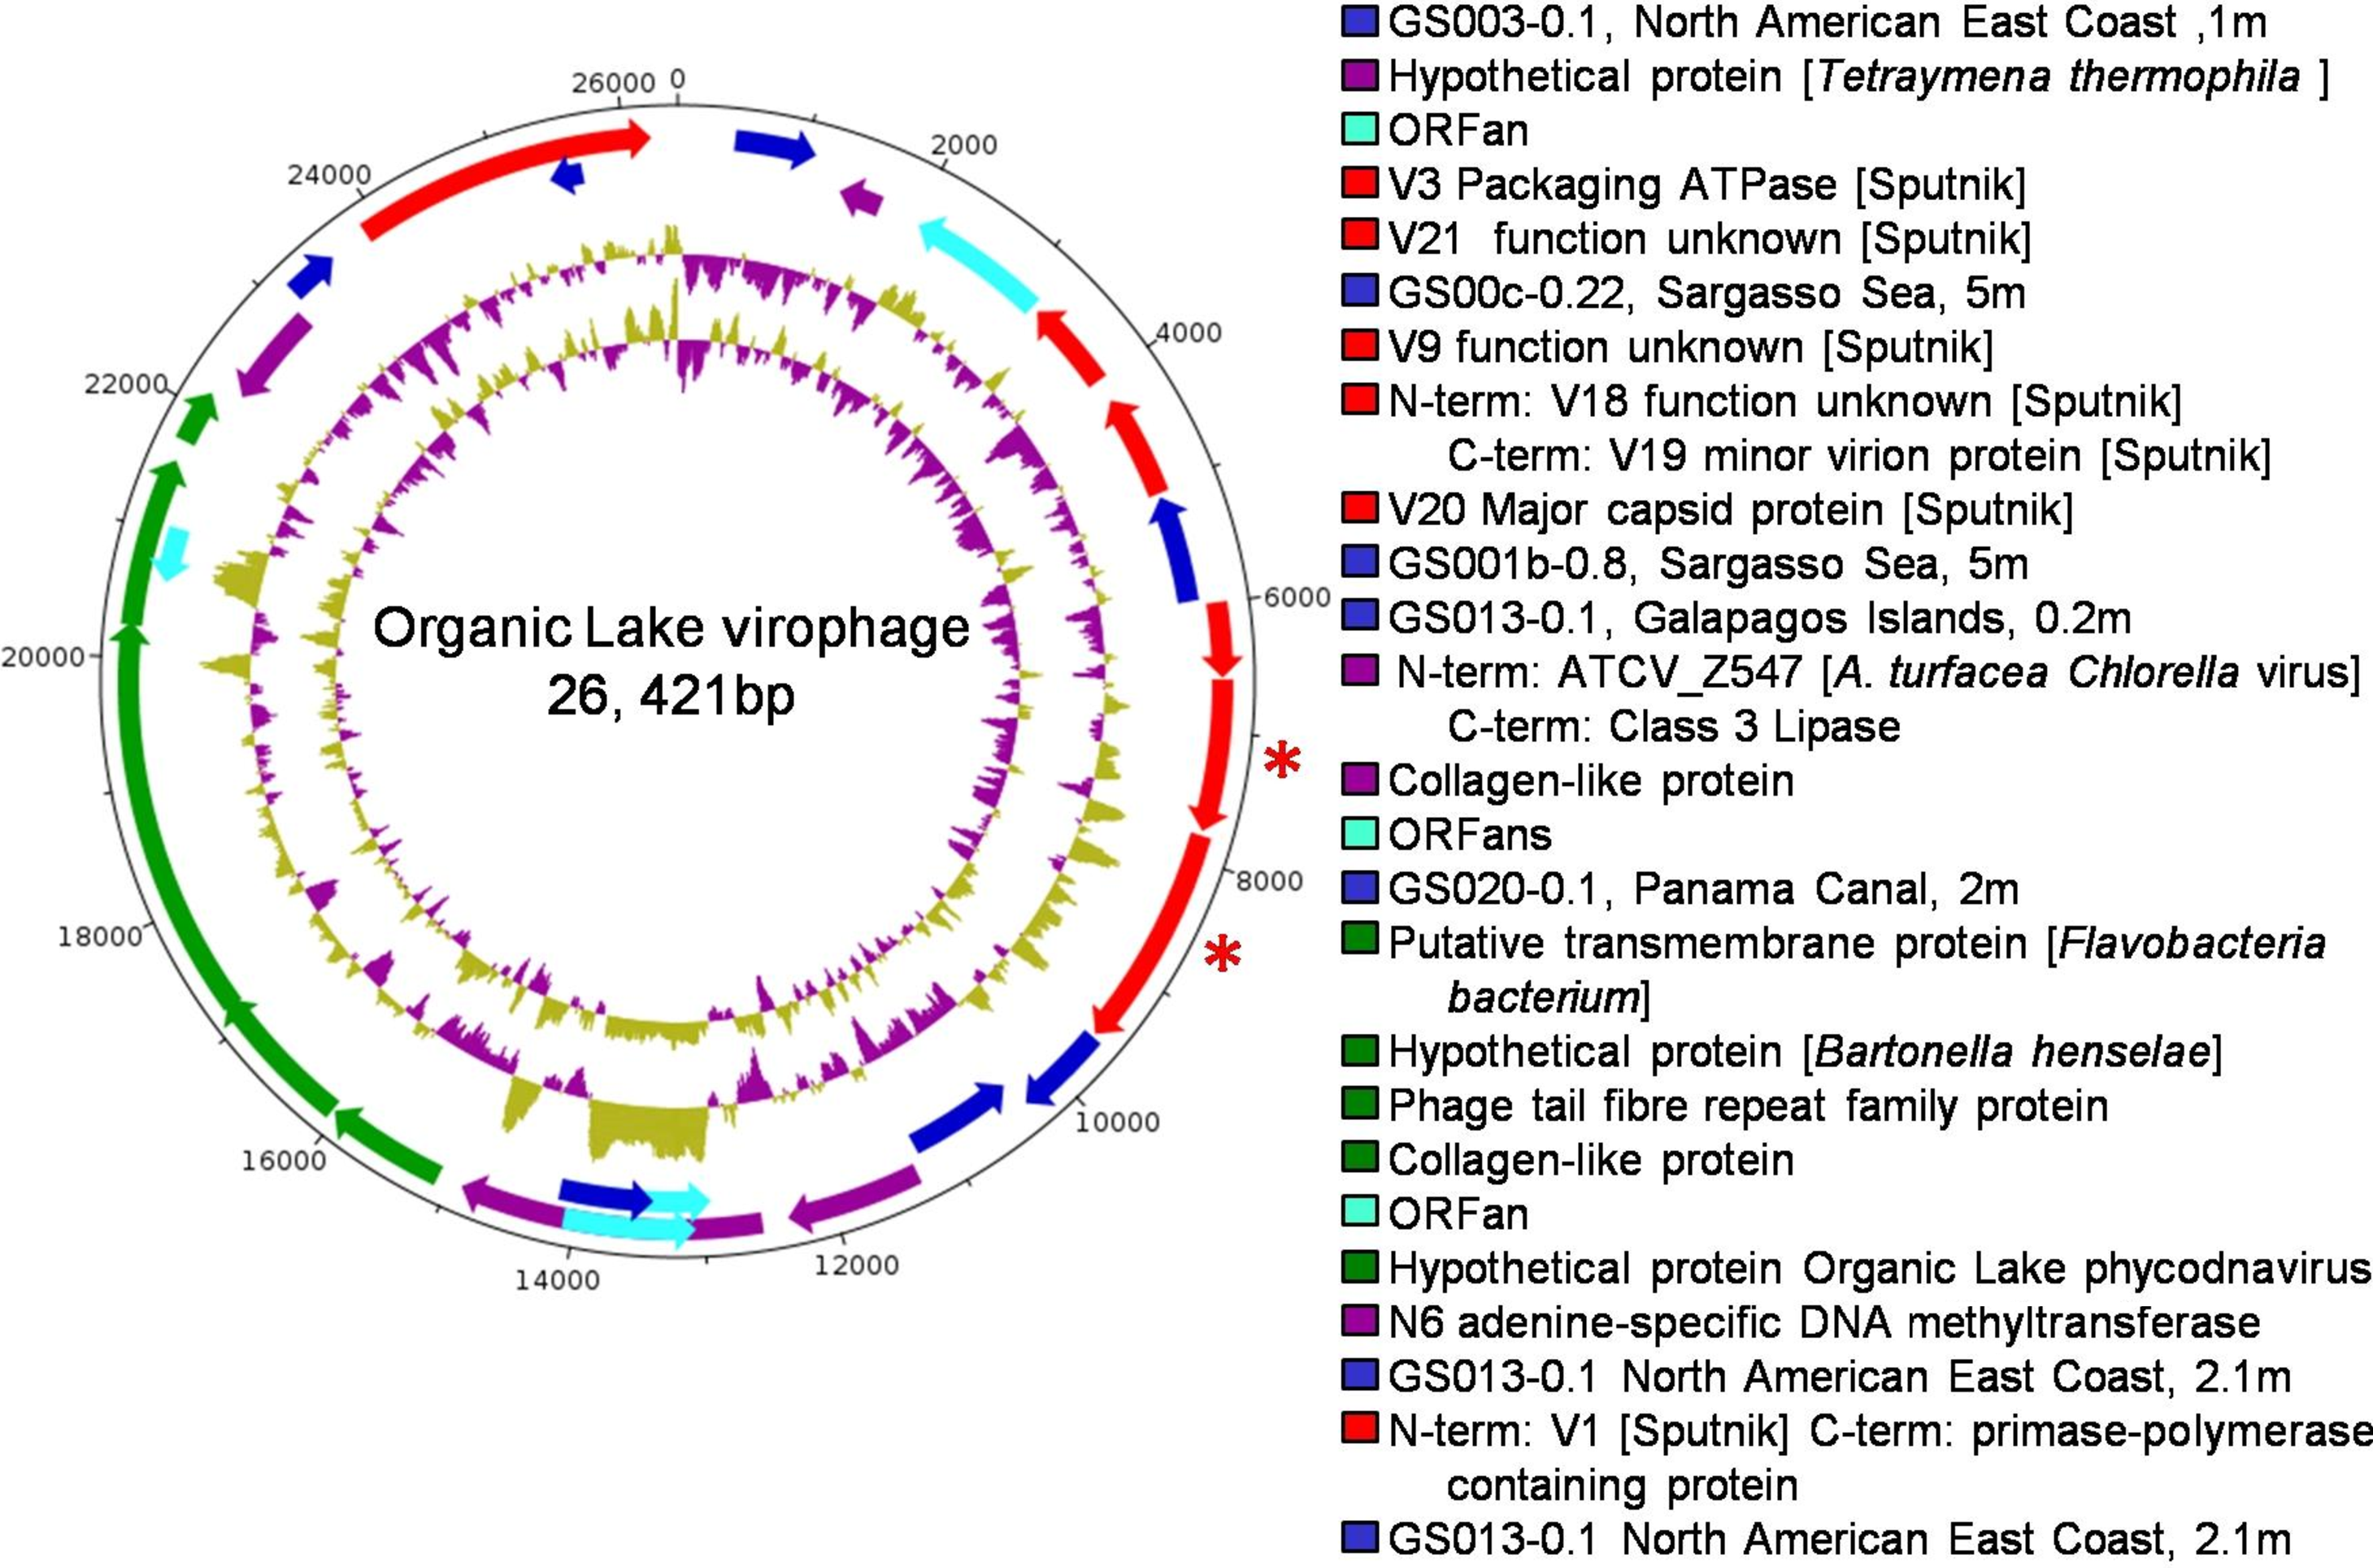
\includegraphics[width=\textwidth]{olv_figures/OLV_genome.pdf}
\caption[Genomic map of Organic Lake virophage]{Genomic map of Organic Lake virophage. From the outside-in, circles represent, 1) predicted coding sequences on the forward strand, 2) predicted coding sequences on the reverse strand, 3) GC skew, and 4) GC plot. Predicted coding sequences are coloured: Sputnik homologues (red), OLPV homologues (green), non-Sputnik \ac{NR} homologues (purple), \ac{GOS} peptide database homologues (blue), and ORFan (cyan). Sequences identified in the metaproteome are marked with an asterisk. Descriptions of the predicted coding sequences from both strands are shown clockwise from position zero.
}
\label{fig:OLV_genome}

\end{figure}
